\documentclass{article}

% chinese fonts
\usepackage{ctex}

% math fonts
\usepackage{amsmath}
\usepackage{amsthm}
\usepackage{amssymb}
\usepackage{bm}

% figures
\usepackage{tikz}
\usepackage{graphicx}
\graphicspath{{./figures/}}

% tables
\usepackage{tabularx}
\usepackage{booktabs}

% codes
\usepackage{listings}
\lstset{language     = Matlab,
        basicstyle   = \ttfamily,
        keywordstyle = \color{cyan},
        rulecolor    = \color{black},
        commentstyle = \color{green},
        keepspaces   = true,
        tabsize      = 4,
}

% hyperlinks
\usepackage{hyperref}
\hypersetup{
  breaklinks,
  colorlinks = true,
  citecolor  = blue,
  linkcolor  = red,
  urlcolor   = magenta,
}

% algorithms
\usepackage{algorithm}
\usepackage{algorithmic}

% bibliography
\usepackage[sort&compress,numbers]{natbib}

% About:  Macros for Vector, Matrix, Tensor, Math Operator and Misc
% Author: Jingxuan Yang

% vectors
\newcommand{\va}{\bm{a}}       \newcommand{\vah}{\hat{\bm{a}}}        \newcommand{\ah}{\hat{a}}    \newcommand{\vat}{\tilde{\bm{a}}}       \newcommand{\at}{\tilde{a}}
\newcommand{\vb}{\bm{b}}       \newcommand{\vbh}{\hat{\bm{b}}}        \newcommand{\bh}{\hat{b}}    \newcommand{\vbt}{\tilde{\bm{b}}}       \newcommand{\bt}{\tilde{b}}
\newcommand{\vc}{\bm{c}}       \newcommand{\vch}{\hat{\bm{c}}}        \newcommand{\ch}{\hat{c}}    \newcommand{\vct}{\tilde{\bm{c}}}       \newcommand{\ct}{\tilde{c}}
\newcommand{\vd}{\bm{d}}       \newcommand{\vdh}{\hat{\bm{d}}}        \newcommand{\dhat}{\hat{d}}  \newcommand{\vdt}{\tilde{\bm{d}}}       \newcommand{\dt}{\tilde{d}}
\newcommand{\ve}{\bm{e}}       \newcommand{\veh}{\hat{\bm{e}}}        \newcommand{\eh}{\hat{e}}    \newcommand{\vet}{\tilde{\bm{e}}}       \newcommand{\et}{\tilde{e}}
\newcommand{\vf}{\bm{f}}       \newcommand{\vfh}{\hat{\bm{f}}}        \newcommand{\fh}{\hat{f}}    \newcommand{\vft}{\tilde{\bm{f}}}       \newcommand{\ft}{\tilde{f}}
\newcommand{\vg}{\bm{g}}       \newcommand{\vgh}{\hat{\bm{g}}}        \newcommand{\gh}{\hat{g}}    \newcommand{\vgt}{\tilde{\bm{g}}}       \newcommand{\gt}{\tilde{g}}
\newcommand{\vh}{\bm{h}}     \newcommand{\vhh}{\hat{\bm{h}}}        \newcommand{\hh}{\hat{h}}    \newcommand{\vht}{\tilde{\bm{h}}}       \newcommand{\htild}{\tilde{h}}
\newcommand{\vi}{\bm{i}}       \newcommand{\vih}{\hat{\bm{i}}}        \newcommand{\ih}{\hat{i}}    \newcommand{\vit}{\tilde{\bm{i}}}       \newcommand{\itild}{\tilde{i}}
\newcommand{\vj}{\bm{j}}       \newcommand{\vjh}{\hat{\bm{j}}}        \newcommand{\jh}{\hat{j}}    \newcommand{\vjt}{\tilde{\bm{j}}}       \newcommand{\jt}{\tilde{j}}
\newcommand{\vk}{\bm{k}}       \newcommand{\vkh}{\hat{\bm{k}}}        \newcommand{\kh}{\hat{k}}    \newcommand{\vkt}{\tilde{\bm{k}}}       \newcommand{\kt}{\tilde{k}}
\newcommand{\vl}{\bm{l}}       \newcommand{\vlh}{\hat{\bm{l}}}        \newcommand{\lh}{\hat{l}}    \newcommand{\vlt}{\tilde{\bm{l}}}       \newcommand{\lt}{\tilde{l}}
\newcommand{\vm}{\bm{m}}       \newcommand{\vmh}{\hat{\bm{m}}}        \newcommand{\mh}{\hat{m}}    \newcommand{\vmt}{\tilde{\bm{m}}}       \newcommand{\mt}{\tilde{m}}
\newcommand{\vn}{\bm{n}}       \newcommand{\vnh}{\hat{\bm{n}}}        \newcommand{\nh}{\hat{n}}    \newcommand{\vnt}{\tilde{\bm{n}}}       \newcommand{\nt}{\tilde{n}}
\newcommand{\vo}{\bm{o}}       \newcommand{\voh}{\hat{\bm{o}}}        \newcommand{\oh}{\hat{o}}    \newcommand{\vot}{\tilde{\bm{o}}}       \newcommand{\ot}{\tilde{o}}
\newcommand{\vp}{\bm{p}}       \newcommand{\vph}{\hat{\bm{p}}}        \newcommand{\ph}{\hat{p}}    \newcommand{\vpt}{\tilde{\bm{p}}}       \newcommand{\pt}{\tilde{p}}
\newcommand{\vq}{\bm{q}}       \newcommand{\vqh}{\hat{\bm{q}}}        \newcommand{\qh}{\hat{q}}    \newcommand{\vqt}{\tilde{\bm{q}}}       \newcommand{\qt}{\tilde{q}}
\newcommand{\vr}{\bm{r}}       \newcommand{\vrh}{\hat{\bm{r}}}        \newcommand{\rh}{\hat{r}}    \newcommand{\vrt}{\tilde{\bm{r}}}       \newcommand{\rt}{\tilde{r}}
\newcommand{\vs}{\bm{s}}       \newcommand{\vsh}{\hat{\bm{s}}}        \newcommand{\sh}{\hat{s}}    \newcommand{\vst}{\tilde{\bm{s}}}       \newcommand{\st}{\tilde{s}}
\newcommand{\vt}{\bm{t}}       \newcommand{\vth}{\hat{\bm{t}}}        \newcommand{\that}{\hat{t}}  \newcommand{\vtt}{\tilde{\bm{t}}}       \newcommand{\ttil}{\tilde{t}}
\newcommand{\vu}{\bm{u}}       \newcommand{\vuh}{\hat{\bm{u}}}        \newcommand{\uh}{\hat{u}}    \newcommand{\vut}{\tilde{\bm{u}}}       \newcommand{\ut}{\tilde{u}}
\newcommand{\vv}{\bm{v}}       \newcommand{\vvh}{\hat{\bm{v}}}        \newcommand{\vhat}{\hat{v}}    \newcommand{\vvt}{\tilde{\bm{v}}}       \newcommand{\vtild}{\tilde{v}}
\newcommand{\vw}{\bm{w}}       \newcommand{\vwh}{\hat{\bm{w}}}        \newcommand{\wh}{\hat{w}}    \newcommand{\vwt}{\tilde{\bm{w}}}       \newcommand{\wt}{\tilde{w}}
\newcommand{\vx}{\bm{x}}       \newcommand{\vxh}{\hat{\bm{x}}}        \newcommand{\xh}{\hat{x}}    \newcommand{\vxt}{\tilde{\bm{x}}}       \newcommand{\xt}{\tilde{x}}
\newcommand{\vy}{\bm{y}}       \newcommand{\vyh}{\hat{\bm{y}}}        \newcommand{\yh}{\hat{y}}    \newcommand{\vyt}{\tilde{\bm{y}}}       \newcommand{\yt}{\tilde{y}}
\newcommand{\vz}{\bm{z}}       \newcommand{\vzh}{\hat{\bm{z}}}        \newcommand{\zh}{\hat{z}}    \newcommand{\vzt}{\tilde{\bm{z}}}       \newcommand{\zt}{\tilde{z}}

\newcommand{\valpha}{\bm{\alpha}}
\newcommand{\vbeta}{\bm{\beta}}
\newcommand{\vgamma}{\bm{\gamma}}
\newcommand{\vtheta}{\bm{\theta}}
\newcommand{\vlambda}{\bm{\lambda}}
\newcommand{\vmu}{\bm{\mu}}
\newcommand{\vomega}{\bm{\omega}}

\newcommand{\mSigma}{\bm{\Sigma}}

\newcommand{\Fc}{\mathcal{F}}
\newcommand{\Xc}{\mathcal{X}}
\newcommand{\Yc}{\mathcal{Y}}
\newcommand{\Zc}{\mathcal{Z}}
\newcommand{\Gc}{\mathcal{G}}
\newcommand{\Hc}{\mathcal{H}}
\newcommand{\Dc}{\mathcal{D}}
\newcommand{\Cc}{\mathcal{C}}
\newcommand{\Rc}{\mathcal{R}}

% matrices
\newcommand{\ma}{\bm{A}}
\newcommand{\mb}{\bm{B}}
\newcommand{\md}{\bm{D}}
\newcommand{\mH}{\bm{H}}
\newcommand{\mE}{\bm{E}}
\newcommand{\mi}{\bm{I}}
\newcommand{\mk}{\bm{K}}
\newcommand{\ml}{\bm{L}}
\newcommand{\mn}{\bm{N}}
\newcommand{\mP}{\bm{P}}
\newcommand{\mq}{\bm{Q}}
\newcommand{\mr}{\bm{R}}
\newcommand{\mU}{\bm{u}}
\newcommand{\mv}{\bm{v}}
\newcommand{\mw}{\bm{W}}
\newcommand{\mx}{\bm{X}}
\newcommand{\my}{\bm{Y}}
\newcommand{\mz}{\bm{Z}}

% tensors
\newcommand{\tp}{\mathsf{P}}
\newcommand{\tu}{\mathsf{U}}
\newcommand{\tx}{\mathsf{X}}
\newcommand{\ty}{\mathsf{Y}}
\newcommand{\tz}{\mathsf{Z}}
\newcommand{\tw}{\mathsf{W}}
\newcommand{\tf}{\mathsf{F}}
\newcommand{\ta}{\mathsf{A}}
\renewcommand{\th}{\mathsf{H}}

% norms
\newcommand{\mynorm}[2]{\| {#1} \|_{#2}}
\newcommand{\norm}[2]{\mynorm{#1}{#2}}
\newcommand{\bignorm}[2]{\left\| {#1} \right\|_{#2}}
\newcommand{\norml}[1]{\mynorm{#1}{1}}
\newcommand{\bignorml}[1]{\bignorm{#1}{1}}
\newcommand{\infnorm}[1]{\mynorm{#1}{\infty}}
\newcommand{\biginfnorm}[1]{\bignorm{#1}{\infty}}
\newcommand{\oneinf}{\ell_{1,\infty}}
\newcommand{\onetwo}{\ell_{1,2}}
\newcommand{\oneinfnorm}[1]{\mynorm{#1}{1,\infty}}
\newcommand{\bigoneinf}[1]{\bignorm{#1}{1,\infty}}
\newcommand{\onetwonorm}[1]{\mynorm{#1}{1,2}}
\newcommand{\bigonetwo}[1]{\bignorm{#1}{1,2}}
\newcommand{\enorm}[1]{\mynorm{#1}{2}}
\newcommand{\bigenorm}[1]{\bignorm{#1}{2}}
\newcommand{\znorm}[1]{\mynorm{#1}{0}}
\newcommand{\bigznorm}[1]{\bignorm{#1}{0}}
\newcommand{\frob}[1]{\|{#1}\|_{\text{F}}}
\newcommand{\bigfrob}[1]{\bignorm{#1}{\text{F}}}
\newcommand{\grpnorm}[2]{\norm{#1}{\text{Gr}(#2)}}

% math operators
\DeclareMathOperator*{\argmin}{argmin}
\DeclareMathOperator*{\argmax}{argmax}
\DeclareMathOperator{\divg}{div}
\DeclareMathOperator{\dom}{dom}
\DeclareMathOperator{\interior}{int}
\DeclareMathOperator{\ri}{ri}
\DeclareMathOperator{\sgn}{sgn}
\DeclareMathOperator{\trace}{Tr}
\DeclareMathOperator{\diag}{diag}
\DeclareMathOperator{\rank}{rank}
\DeclareMathOperator{\range}{range}
\DeclareMathOperator{\vect}{vec}
\DeclareMathOperator{\prox}{prox}
\DeclareMathOperator{\intr}{int}
\DeclareMathOperator{\relint}{ri}

% misc
\newcommand{\gs}{\geqslant}
\newcommand{\ls}{\leqslant}
\newcommand{\set}[1]{\left\{ {#1}\right\}}

\newcommand{\defeq}{\ \stackrel{\text{def}}{=}\ }
\newcommand{\ip}[2]{\left\langle#1, #2\right\rangle}
\newcommand{\reals}{\mathbb{R}}
\newcommand{\complex}{\mathbb{C}}
\newcommand{\half}{\frac{1}{2}}

\newtheorem{theorem}{Theorem}
\newtheorem{lemma}[theorem]{Lemma}
\newtheorem{proposition}[theorem]{Proposition}
\newtheorem{remark}[theorem]{Remark}
\newtheorem{corollary}[theorem]{Corollary}
\newtheorem{definition}[theorem]{Definition}


\setlength{\oddsidemargin}{-0.25 in}
\setlength{\evensidemargin}{-0.25 in} 
\setlength{\topmargin}{-0.25in} 
\setlength{\textwidth}{7 in} 
\setlength{\textheight}{8.5 in}
\setlength{\headsep}{0.25 in} 
\setlength{\parindent}{0 in}
\setlength{\parskip}{0.1 in}

\newcommand{\homework}[5]{
  \pagestyle{myheadings} 
  \thispagestyle{plain}
  \newpage
  \setcounter{page}{1} 
  \setcounter{section}{#5} 
  \noindent
  \begin{center}
    \framebox{ 
      \vbox{
        \vspace{2mm} 
        \hbox to 6.28in { {\bf
        THU-70250043-0,~Pattern~Recognition~(Spring 2021) \hfill Homework: 4} }
        \vspace{6mm} 
        \hbox to 6.28in { {\Large \hfill #1 \hfill} }
        \vspace{6mm} 
        \hbox to 6.28in { {\it Lecturer: #2 \hfill} }
        \vspace{2mm} 
        \hbox to 6.28in { {\it \hspace{14mm} #3 \hfill} }
        \vspace{2mm} 
        \hbox to 6.28in { {\it Student: #4 \hfill} }
        \vspace{2mm} 
      } 
    }
  \end{center}
  \markboth{#1}{#1} 
  \vspace*{4mm} 
}

\begin{document}

\homework{Overfitting, Error Rate Estimation and Linear Classifiers}{Changshui Zhang
\hspace{5mm} {\tt zcs@mail.tsinghua.edu.cn}}{Hong Zhao \hspace{16mm} {\tt vzhao@tsinghua.edu.cn}}{Jingxuan Yang \hspace{10mm} {\tt yangjx20@mails.tsinghua.edu.cn}}{8}

\section*{Overfitting}

1. Consider $N$ i.i.d. observations $\bm{X}=\{x_1,x_2,\dots,x_N\}$ with corresponding target values $\bm{T}=\{t_1,t_2,\dots,t_N\}$.

We want to fit these observations into a model 
\begin{equation}
  t = y(x, \bm{w}) + \epsilon
\end{equation}
where $\bm{w}$ is the model parameter and $\epsilon$ is the error term.

1.1 To find $\bm{w}$, we can minimize the sum of square error
\begin{equation}
\label{eq0}
E(\bm{w}) = \frac{1}{2} \sum_{n=1}^N \big[y(x_n, \bm{w}) - t_n\big]^2
\end{equation}

Now suppose we believe that the distribution of error term $\epsilon$ is Gaussian 
\begin{equation}
  p(\epsilon | \beta) = \mathcal{N} (\epsilon | 0, \beta^{-1})
\end{equation}
where $\beta=\dfrac{1}{\sigma^2}$ is the inverse of variance. Using the property of Gaussian distribution, we have
\begin{equation}
  p(t|x, \bm{w}, \beta) = \mathcal{N} (t|y(x, \bm{w}), \beta^{-1})
\end{equation}

Under this assumption, the likelihood function is given by 
\begin{equation}
  p(\bm{T}|\bm{X},\bm{w},\beta)=\prod_{n=1}^N \mathcal{N}(t_n|y(x_n,\bm{w}),\beta^{-1})
\end{equation}

Show that the problem of finding the maximum likelihood solution for $\bm{w}$ is equivalent to the problem of minimizing the sum of square error (\ref{eq0}).

解: 对数似然函数为
\begin{equation}
  \begin{aligned}
    H(\bm{\omega})
    &=\ln p(\bm{T}|\bm{X},\bm{w},\beta)\\
    &=\ln\left[\prod_{n=1}^N \mathcal{N}(t_n|y(x_n,\bm{w}),\beta^{-1})\right]\\
    &=\sum_{n=1}^N\ln\mathcal{N}(t_n|y(x_n,\bm{w}),\beta^{-1})\\
    &=\sum_{n=1}^N\ln\left[\frac{1}{\sqrt{2\pi\beta^{-1}}}\exp\left(-\frac{[t_n-y(x_n,\bm{w})]^2}{2\beta^{-1}}\right)\right]\\
    &=\sum_{n=1}^N\left(\ln\frac{1}{\sqrt{2\pi\beta^{-1}}}-\frac{\beta}{2}[t_n-y(x_n,\bm{w})]^2\right)\\
    &=-N\ln\sqrt{2\pi\beta^{-1}}-\frac{\beta}{2}\sum_{n=1}^N[t_n-y(x_n,\bm{w})]^2
  \end{aligned}
\end{equation}

所以, $\bm{w}$ 的最大似然估计为
\begin{equation}
  \hat{\bm{w}}\in\argmax_{\bm{w}}\left\{-N\ln\sqrt{2\pi\beta^{-1}}-\frac{\beta}{2}\sum_{n=1}^N[t_n-y(x_n,\bm{w})]^2\right\}
\end{equation}

忽略第一项常数项, 上述问题等价于
\begin{equation}
  \hat{\bm{w}}\in\argmax_{\bm{w}}\left\{-\frac{\beta}{2}\sum_{n=1}^N[t_n-y(x_n,\bm{w})]^2\right\}
\end{equation}

又 $\beta>0$, 则有
\begin{equation}
  \label{eq:mle}
  \hat{\bm{w}}\in\argmin_{\bm{w}}\left\{\frac{1}{2}\sum_{n=1}^N[t_n-y(x_n,\bm{w})]^2\right\}
\end{equation}

对最小二乘法, 有
\begin{equation}
  \label{eq:mse}
  \tilde{\bm{w}}\in\argmin_{\bm{w}}\left\{\frac{1}{2}\sum_{n=1}^N[y(x_n,\bm{w})-t_n]^2\right\}
\end{equation}

比较式 (\ref{eq:mle}) 与式 (\ref{eq:mse}) 可知 $\tilde{\bm{w}}=\hat{\bm{w}}$, 即最大似然估计与最小二乘的结果等价.

1.2 In order to avoid overfitting, we often add a weight decay term to (\ref{eq0})
\begin{equation}
  \label{eq1}
  \tilde{E}(\bm{w})=\frac{1}{2}\sum_{n=1}^N\big[y(x_n,\bm{w})-t_n\big]^2
  +\frac{\lambda}{2} \|\bm{w}\|_2^2
\end{equation}

On the other hand, we believe that $\bm{w}$ has a prior distribution of 
\[
p(\bm{w} | \alpha) = \mathcal{N} (\bm{w} | \bm{0}, \alpha^{-1} \bm{I})
\]

Using Bayes theorem, the posterior distribution for $\bm{w}$ is proportional to the product of the prior distribution and the likelihood function
\begin{equation}
\label{eq2}
p(\bm{w} | \bm{X}, \bm{T}, \alpha, \beta) \propto 
p(\bm{T} | \bm{X}, \bm{w}, \beta) p(\bm{w} | \alpha)
\end{equation}

Show that the problem of finding Maximum A Posterior (MAP) solution for $\bm{w}$ (i.e., maximizing (\ref{eq2})) is equivalent to the problem of minimizing (\ref{eq1}).

解: 令
\begin{equation}
  \begin{aligned}
    \tilde{H}(\bm{\omega})
    &\triangleq\ln\big[p(\bm{T} | \bm{X}, \bm{w}, \beta) p(\bm{w}|\alpha)\big]\\
    &=\ln\left[\prod_{n=1}^N \mathcal{N}(t_n|y(x_n,\bm{w}),\beta^{-1})p(\bm{w}|\alpha)\right]\\
    &=\sum_{n=1}^N\ln\mathcal{N}(t_n|y(x_n,\bm{w}),\beta^{-1})+\ln p(\bm{w}|\alpha)\\
    &=\sum_{n=1}^N\left(\ln\frac{1}{\sqrt{2\pi\beta^{-1}}}-\frac{[t_n-y(x_n,\bm{w})]^2}{2\beta^{-1}}\right)+\ln\frac{1}{\sqrt{2\pi\alpha^{-1}}}-\frac{\|\bm{w}\|_2^2}{2\alpha^{-1}}\\
    &=-N\ln\sqrt{2\pi\beta^{-1}}-\ln\sqrt{2\pi\alpha^{-1}}-\frac{\beta}{2}\sum_{n=1}^N[t_n-y(x_n,\bm{w})]^2-\frac{\alpha}{2}\|\bm{w}\|_2^2\\
  \end{aligned}
\end{equation}

所以, $\bm{w}$ 的最大后验估计 (MAP) 为
\begin{equation}
  \hat{\bm{w}}\in\argmax_{\bm{w}}\left\{-N\ln\sqrt{2\pi\beta^{-1}}-\ln\sqrt{2\pi\alpha^{-1}}-\frac{\beta}{2}\sum_{n=1}^N[t_n-y(x_n,\bm{w})]^2-\frac{\alpha}{2}\|\bm{w}\|_2^2\right\}
\end{equation}

忽略常数项, 上述问题等价于
\begin{equation}
  \hat{\bm{w}}\in\argmax_{\bm{w}}\left\{-\frac{\beta}{2}\sum_{n=1}^N[t_n-y(x_n,\bm{w})]^2-\frac{\alpha}{2}\|\bm{w}\|_2^2\right\}
\end{equation}

又 $\beta>0$, 则有
\begin{equation}
  \label{eq:map}
  \hat{\bm{w}}\in\argmin_{\bm{w}}\left\{\frac{1}{2}\sum_{n=1}^N[t_n-y(x_n,\bm{w})]^2+\frac{\alpha}{2\beta}\|\bm{w}\|_2^2\right\}
\end{equation}

对加入正则项的最小二乘法, 有
\begin{equation}
  \label{eq:mser}
  \tilde{\bm{w}}\in\argmin_{\bm{w}}\left\{\frac{1}{2}\sum_{n=1}^N[y(x_n,\bm{w})-t_n]^2+\frac{\lambda}{2} \|\bm{w}\|_2^2\right\}
\end{equation}

比较式 (\ref{eq:map}) 与式 (\ref{eq:mser}) 可知, 当 $\lambda=\dfrac{\alpha}{\beta}$ 时, 有 $\tilde{\bm{w}}=\hat{\bm{w}}$, 即最大后验估计与正则化最小二乘的结果等价.

\section*{Programming for Error Rate Estimation}

2. Consider a two dimensional classification problems: $p(\omega_{1})=p(\omega_{2})= 0.5$, $p(x|\omega_{1}) \sim N(\mu_{1},\Sigma_{1})$, $p(x|\omega_{2}) \sim N(\mu_{2},\Sigma_{2})$, where
\begin{equation}
  \mu_1=
    \begin{bmatrix}
      -1 \\ 
      0 \\
    \end{bmatrix},~
  \mu_2=
    \begin{bmatrix}
      1 \\ 
      0 \\
    \end{bmatrix},\quad
  \Sigma_1=
    \begin{bmatrix}
      1 & 0 \\
      0 & 1 \\
    \end{bmatrix},~
  \Sigma_2=
    \begin{bmatrix}
      1 & 0 \\
      0 & 1 \\
    \end{bmatrix}
\end{equation}

2.1 Derive the misclassification rate of the Bayesian classifier theoretically.

解: Bayes 决策边界满足
\begin{equation}
  p(x|\omega_{1})p(\omega_{1})=p(x|\omega_{2})p(\omega_{2})
\end{equation}

即
\begin{equation}
  \frac{1}{2}\frac{1}{2\pi}\exp\left[-\frac{(x_1+1)^2+x_2^2}{2}\right]=\frac{1}{2}\frac{1}{2\pi}\exp\left[-\frac{(x_1-1)^2+x_2^2}{2}\right]
\end{equation}

化简得
\begin{equation}
  x_1=0
\end{equation}

所以, 错误率为
\begin{equation}
  \begin{aligned}
    P(e)
    &=\int_{-\infty}^\infty\int_{-\infty}^0 p(x|\omega_{2})p(\omega_{2})\mathrm{d}x_1\mathrm{d}x_2+\int_{-\infty}^\infty\int_0^\infty p(x|\omega_{1})p(\omega_{1})\mathrm{d}x_1\mathrm{d}x_2\\
    &=\int_{-\infty}^\infty\int_{-\infty}^0\frac{1}{2}\frac{1}{2\pi}\exp\left[-\frac{(x_1-1)^2+x_2^2}{2}\right]\mathrm{d}x_1\mathrm{d}x_2+\int_{-\infty}^\infty\int_0^\infty\frac{1}{2}\frac{1}{2\pi}\exp\left[-\frac{(x_1+1)^2+x_2^2}{2}\right]\mathrm{d}x_1\mathrm{d}x_2\\
    &=\int_{-\infty}^\infty\int_{-\infty}^0\frac{1}{2\pi}\exp\left[-\frac{(x_1-1)^2+x_2^2}{2}\right]\mathrm{d}x_1\mathrm{d}x_2\\
    &=\int_{-\infty}^0\frac{1}{\sqrt{2\pi}}\exp\left[-\frac{(x_1-1)^2}{2}\right]\mathrm{d}x_1\\
    &=\Phi(-1)\\
    &=0.1587\\
  \end{aligned}
\end{equation}

2.2 Choose a proper $n$ and draw $n$ samples from $p(x|\omega_{1})$ and $p(x|\omega_{2})$ with labels respectively. Estimate $p_{n}(x|\omega_{1})$ and $p_{n}(x|\omega_{2})$ by Parzen window method, with Gaussian window function and unit hypercube window function. Design Bayesian classifier with your estimated $p_{n}(x|\omega_{1})$ and $p_{n}(x|\omega_{2})$. Compare their misclassification rate with the theoretical optimal Bayesian classifier in theory.

解: 取 $n=1000$, 使用二维高斯核函数
\begin{equation}
  K(x)=\frac{1}{2\pi a^2}\exp\left(-\frac{\|x\|_2^2}{2a^2}\right)
\end{equation}

进行估计, 取窗宽 $a=[0.01,10]$, 做出高斯估计均方误差与窗宽的变化曲线如图 \ref{fig:mseGaussian} 所示, 由图可以得出 $n=1000$ 时高斯估计的最优窗宽为 $a=0.3$. 在最优窗宽的情况下做 10 次估计, 得到平均均方误差为
\begin{equation}
  \epsilon(p_n(x|\omega_1))=0.0011,\quad\epsilon(p_n(x|\omega_2))=0.0011
\end{equation}

\begin{figure}[tbp]
  \centering
  \begin{minipage}[t]{0.48\textwidth}
  \centering
  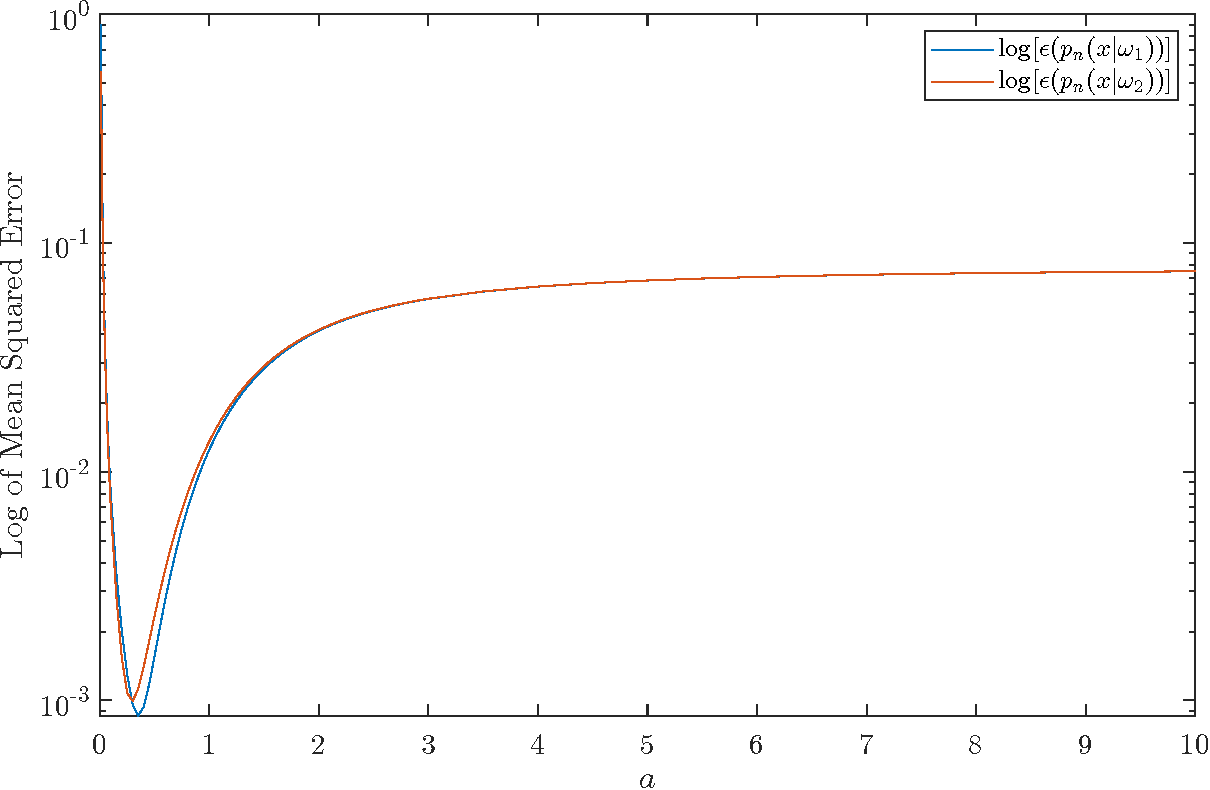
\includegraphics[width=8cm]{mseGaussian.pdf}
  \caption{高斯估计均方误差与窗宽变化关系}
  \label{fig:mseGaussian}
  \end{minipage}
  \begin{minipage}[t]{0.48\textwidth}
  \centering
  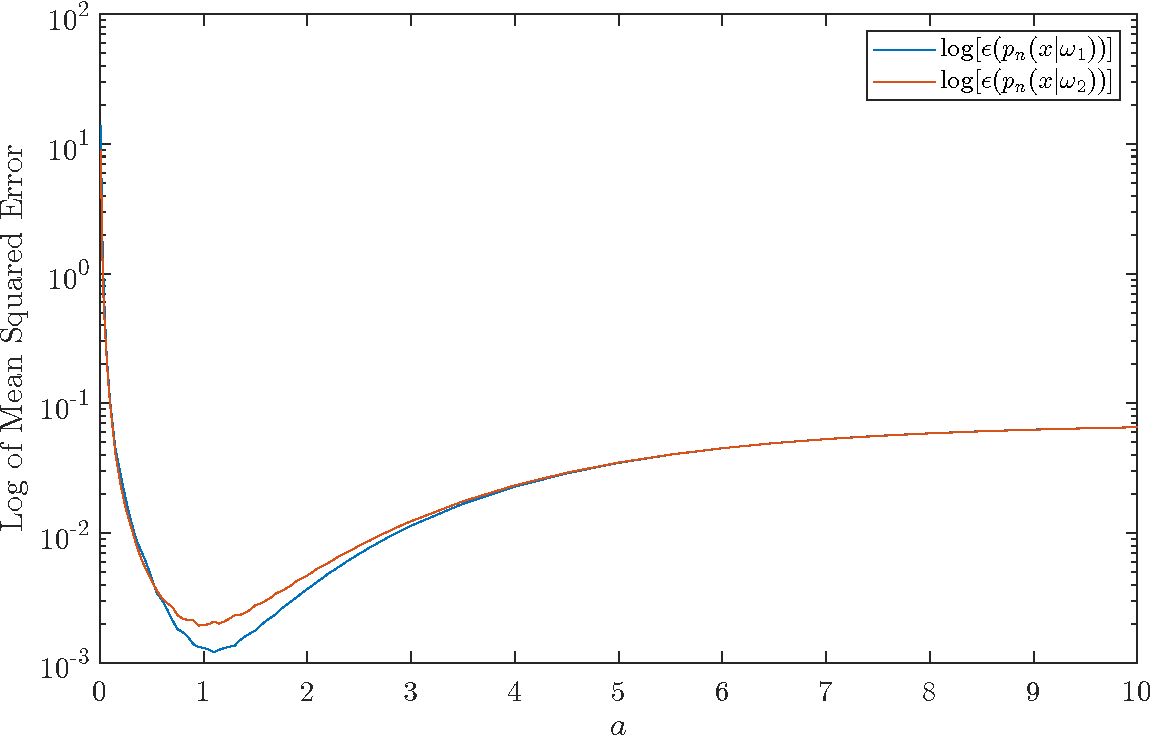
\includegraphics[width=8cm]{mseCube.pdf}
  \caption{方窗估计均方误差与窗宽变化关系}
  \label{fig:mseCube}
  \end{minipage}
\end{figure}

使用二维方窗核函数
\begin{equation}
  K(x)=
  \left\{
    \begin{array}{ll}
      \dfrac{1}{a^2},& \|x\|_\infty \ls\dfrac{a}{2} \\
      0, & \text{otherwise.}
    \end{array}
  \right.
\end{equation}

进行估计, 同样取 $a=[0.01,10]$, 做出方窗估计均方误差与窗宽的变化曲线如图 \ref{fig:mseCube} 所示, 由图可以得出 $n=1000$ 时方窗估计的最优窗宽为 $a=1$. 在最优窗宽的情况下做 10 次估计, 得到平均均方误差为
\begin{equation}
  \epsilon(p_n(x|\omega_1))=0.0012,\quad\epsilon(p_n(x|\omega_2))=0.0010
\end{equation}

由于 $p(\omega_{1})=p(\omega_{2})= 0.5$, 则 Bayes 分类器为
\begin{equation}
  \begin{aligned}
    p_n(x|\omega_1) > p_n(x|\omega_2) &\to x\in\omega_1\\
    p_n(x|\omega_2) > p_n(x|\omega_1) &\to x\in\omega_2\\
  \end{aligned}
\end{equation}

在最优窗宽的情况下做 10 次估计, 高斯估计和方窗估计的错误率分别如表 \ref{tab:gaussianErr} 和表 \ref{tab:rectErr} 所示, 平均错误率为
\begin{equation}
  \bar{P}_{\mathrm{Guassian}}(e)=0.1569,\quad \bar{P}_{\mathrm{hypercube}}(e)=0.1587
\end{equation}

理论上, 当样本数量 $n\to\infty$ 时, Parzen 窗法得到的概率密度函数估计是没有偏差的, 则错误率也与 Bayes 理论错误率相同. 但是实际估计时样本数量有限, 估计的概率密度函数与理论值之间存在偏差, 则 Parzen 窗法错误率也与 Bayes 理论错误率存在偏差. 通过实验数据比较两种 Parzen 窗法和 Bayes 的理论错误率, 可以看出方窗的平均错误率与 Bayes 理论错误率几乎相同, 高斯窗的平均错误率比 Bayes 理论错误率略小一些.

\begin{table}[htbp]
  \centering
  \begin{minipage}{0.4\textwidth}
    \centering
    \caption{高斯窗估计错误率}
    \label{tab:gaussianErr}
    \begin{tabular}{c|ccc}
      \hline
      No. & $P_1(e)$ & $P_2(e)$ & $P(e)$ \\
      \hline
      1  & 0.1389 & 0.1746 & 0.1568 \\
      2  & 0.1641 & 0.1493 & 0.1567 \\
      3  & 0.1672 & 0.1493 & 0.1582 \\
      4  & 0.1392 & 0.1754 & 0.1573 \\
      5  & 0.1623 & 0.1510 & 0.1566 \\
      6  & 0.1611 & 0.1516 & 0.1563 \\
      7  & 0.1518 & 0.1624 & 0.1571 \\
      8  & 0.1568 & 0.1568 & 0.1568 \\
      9  & 0.1634 & 0.1495 & 0.1564 \\
      10 & 0.1446 & 0.1694 & 0.1570 \\
      \hline   
    \end{tabular}
  \end{minipage}
  \begin{minipage}{0.4\textwidth}
    \centering
    \caption{方窗估计错误率}
    \label{tab:rectErr}
    \begin{tabular}{c|ccc}
      \hline
      No. & $P_1(e)$ & $P_2(e)$ & $P(e)$ \\
      \hline
      1  & 0.1671 & 0.1507 & 0.1589 \\
      2  & 0.1495 & 0.1671 & 0.1583 \\
      3  & 0.1642 & 0.1510 & 0.1576 \\
      4  & 0.1609 & 0.1549 & 0.1579 \\
      5  & 0.1748 & 0.1426 & 0.1587 \\
      6  & 0.1434 & 0.1733 & 0.1584 \\
      7  & 0.1549 & 0.1621 & 0.1585 \\
      8  & 0.1304 & 0.1898 & 0.1601 \\
      9  & 0.1632 & 0.1538 & 0.1585 \\
      10 & 0.1699 & 0.1497 & 0.1598 \\
      \hline
    \end{tabular}
  \end{minipage}
\end{table}

2.3 From above experiments, what's your suggestion for choosing optimal window function and parameters with given $n$?

解: 建议选择窗函数和窗宽参数时, 根据估计的概率密度函数的均方误差和相应的错误率来选择, 综合选择均方误差较小且错误率也较小的窗函数和窗宽参数. 根据上述实验结果可知, 本实验中若选择高斯函数, 且最优窗宽选择 $a=0.3$, 则此时估计的均方误差和错误率相对于其他测试参数而言都是最小的.

2.4 Sample $2n$ points from the Gaussian mixture distribution $p(x)$ without labels. Use EM to estimate $\mu_{1}$, $\mu_{2}$, $\Sigma_{1}$, $\Sigma_{2}$ so that we estimate $p_{2n}(x|\omega_{1})$ and $p_{2n}(x|\omega_{2})$. Which method is more accurate in estimating $p(x|\omega_{1})$ and $p(x|\omega_{2})$, EM or Parzen window? Prove your statement by experiments.

解: 使用 EM 算法估计 10 次, 其中似然概率最大的一组估计结果为
\begin{equation}
  \hat{\mu}_1=
    \begin{bmatrix}
      -1.0212 \\ 
      -0.0259 \\
    \end{bmatrix},~
  \hat{\mu}_2=
    \begin{bmatrix}
      0.9645 \\ 
      -0.0234 \\
    \end{bmatrix},\quad
  \hat{\Sigma}_1=
    \begin{bmatrix}
      1.0156 & -0.0165 \\
      -0.0165 & 1.0035 \\
    \end{bmatrix},~
  \hat{\Sigma}_2=
    \begin{bmatrix}
      1.0156 & -0.0165 \\
      -0.0165 & 1.0035 \\
    \end{bmatrix}
\end{equation}

且估计的均方误差为
\begin{equation}
  \epsilon(p_{2n}(x|\omega_1))=0.0003,\quad \epsilon(p_{2n}(x|\omega_2))=0.0009
\end{equation}

通过均方误差的比较来看, EM 算法最好的估计结果比两种 Parzen 窗的估计效果都更加精确.

2.5 Design Bayesian classifier with the estimated $p_{2n}(x|\omega_{1})$ and $p_{2n}(x|\omega_{2})$ by EM. Analyze its performance, i.e., the expectation and variance of misclassification rate and compare them with that of optimal Bayesian classifier.

解: 由于 $p(\omega_{1})=p(\omega_{2})= 0.5$, 则 Bayes 分类器为
\begin{equation}
  \begin{aligned}
    p_{2n}(x|\omega_1) > p_{2n}(x|\omega_2) &\to x\in\omega_1\\
    p_{2n}(x|\omega_2) > p_{2n}(x|\omega_1) &\to x\in\omega_2\\
  \end{aligned}
\end{equation}

使用 EM 算法估计 10 次, 错误率如表 \ref{tab:emErr} 所示.

\begin{table}[htbp]
  \centering
  \caption{EM 算法估计错误率}
  \label{tab:emErr}
  \begin{tabular}{c|ccc}
    \hline
    No. & $P_1(e)$ & $P_2(e)$ & $P(e)$ \\
    \hline
    1  & 0.2229  & 0.3611 & 0.2920 \\
    2  & 0.1777  & 0.1732 & 0.1754 \\
    3  & 0.1819  & 0.1695 & 0.1757 \\
    4  & 0.1546  & 0.1570 & 0.1558 \\
    5  & 0.1611  & 0.1504 & 0.1557 \\
    6  & 0.2014  & 0.2941 & 0.2478 \\
    7  & 0.1749  & 0.1480 & 0.1615 \\
    8  & 0.1582  & 0.1528 & 0.1555 \\
    9  & 0.1782  & 0.1728 & 0.1755 \\
    10 & 0.1552  & 0.1563 & 0.1558 \\
    \hline  
  \end{tabular}
\end{table}

错误率的期望和方差分别为
\begin{equation}
  \mathbb{E}[P(e)]=0.1851,\quad \mathrm{Var}[P(e)]=0.0022
\end{equation}

由实验结果可知, EM 算法的平均错误率比 Bayes 分类的理论错误率高, 方差较小但还是有一些, 主要是因为 EM 算法偶尔会收敛到局部最优解.

2.6 Conclude your results. Which method is your favorite to estimate parameters and which classifier is your favorite classifier? Why?

解: 这个实验内容包含了之前所学的统计决策方法和概率密度函数的估计两部分内容. 首先, 在概率分布模型以及参数都已知时, 可以直接使用 Bayes 分类, 得到最小错误率的分类器. 若已知概率分布模型, 但是不知道具体参数值, 则可以选择 EM 算法等参数方法进行参数估计, 再进行 Bayes 分类; 当概率分布模型也未知时, 可以选用 Parzen 窗等非参数方法进行估计, 之后进行 Bayes 分类.

相对而言, 我更倾向于选择 EM 算法等参数化方法来估计概率模型的参数并使用 Bayes 分类器, 这是因为 Parzen 窗等非参数方法存在维数爆炸的问题, 同时运算量很大, 还要选择合适的窗函数以及最优窗宽大小; 而参数方法相对比较简单, 且运算量更小.

\newpage
\section*{Programming for Single Sample Correction Algorithm}

3. The training process of the Single Sample Correction Algorithm (Algorithm~\ref{alg:1}) can be regarded as a searching process for a solution in feasible solution region, whereas no strict restrictions are demanded for the capacity of this solution. The solution only needs to satisfy $a^{\top}y_n>0$, where $a$ is the weight vector of the perceptron, and $y_n$ is the normalized augmented sample vector. However, the margin perceptron (Algorithm~\ref{alg:2}) requires the finally converged hyperplane possesses a margin ($>\gamma$), where $\gamma$ is a predefined positive scalar. It means that the final solution of perceptron need to satisfy $a^{\top}y_n>\gamma$.

Thus, there are two types of ``mistakes'' during the training of perceptron, namely (1) the prediction mistake and (2) margin mistake (i.e., its prediction is correct, but its margin is not large enough).

\begin{algorithm}[htb]
  \caption{Fixed-Increment Single Sample Correction Algorithm}
  \label{alg:1}
  \begin{algorithmic}[1]
  \STATE \textbf{initialize} $a$, $k\gets0$
  \REPEAT
    \STATE $k\gets(k+1)$ mod $n$
    \IF{$y_k$ is misclassified by $a$}
        \STATE $a\gets a+y_k$
    \ENDIF
  \UNTIL {all patterns are properly classified}
  \STATE \textbf{return} $a$
  \end{algorithmic}
\end{algorithm}

\begin{algorithm}[htb]
  \caption{Single Sample Correction Algorithm With Margin}
  \label{alg:2}
  \begin{algorithmic}[1]
  \STATE \textbf{initialize} $a$, $k\gets0,~\gamma>0$
  \REPEAT
    \STATE $k\gets(k+1)$ mod $n$
    \IF{$a^{\top}y_k\ls\gamma$}
        \STATE $a\gets a+y_k$
    \ENDIF
  \UNTIL {all patterns are properly classified with a large enough margin $\gamma$}
  \STATE \textbf{return} $a$
  \end{algorithmic}
\end{algorithm}

3.1 Please generate 200 data points in the 2D plane, among which 100 data points are labeled as 1 and the remaining 100 are labeled as $-1$. Make sure that these 200 data points are linearly separable. Plot these 200 data points in a 2D plane.

解: 设定超平面保证两类数据点线性可分, 生成的 200 个数据点保存在 \verb|percepData.mat| 文件, 如图 \ref{fig:dataPoints} 所示.

\begin{figure}[tbp]
  \centering
  \begin{minipage}[t]{0.48\textwidth}
  \centering
  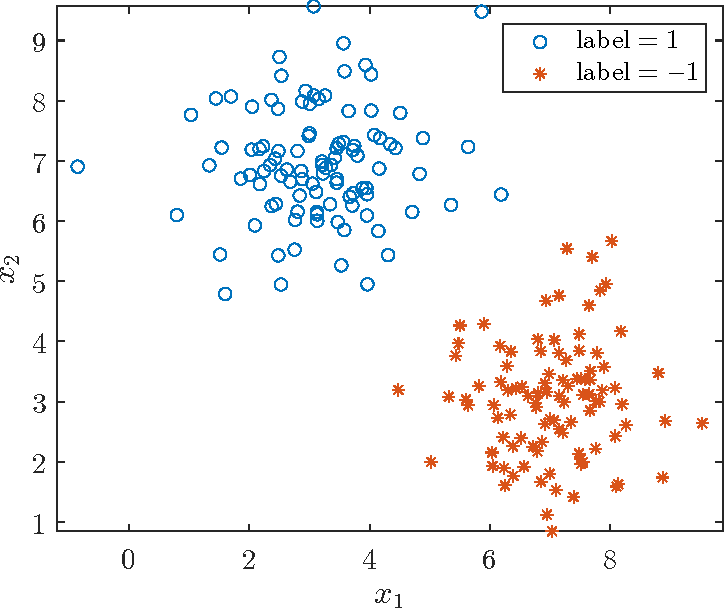
\includegraphics[width=8cm]{dataPoints.pdf}
  \caption{200 个数据点, 分为两类}
  \label{fig:dataPoints}
  \end{minipage}
  \begin{minipage}[t]{0.48\textwidth}
  \centering
  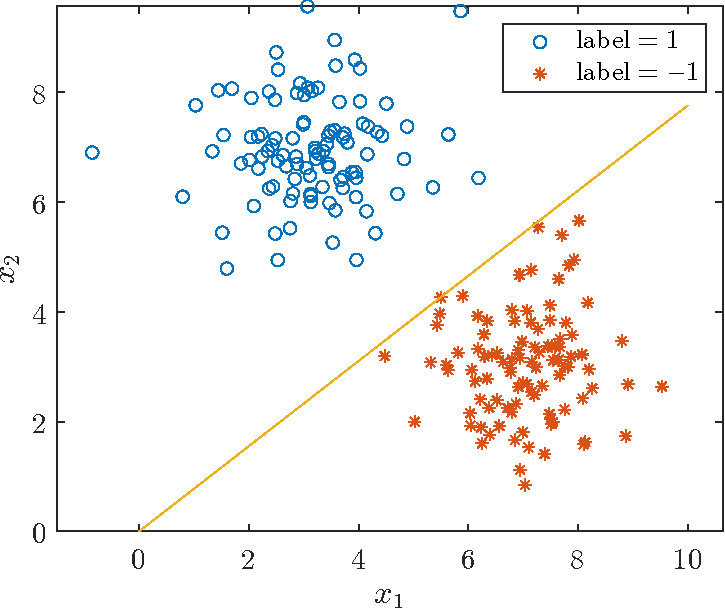
\includegraphics[width=8cm]{classicalPrecep.pdf}
  \caption{经典感知器分类结果}
  \label{fig:classicalPrecep}
  \end{minipage}
\end{figure}

3.2 Implement the classical perceptron algorithm and run it on the above generated data points. Plot the classification boundary and these data points in one figure.

解: 经典感知器的分类边界如图 \ref{fig:classicalPrecep} 所示.

3.3 Implement the margin perceptron algorithm and run it on the above generated data points. Plot the classification boundary and these data points in one figure. Analyze the impacts of $\gamma$ on algorithm convergence and the classification boundary.

解: 取 $\gamma=10$, margin 感知器的分类边界如图 \ref{fig:marginPrecep} 所示. 

$\gamma$ 大小对算法迭代次数的影响如图 \ref{fig:marginEffect} 所示, 可知随着 $\gamma$ 的增大, 算法迭代次数不断震荡波动但是大体上逐渐增加, 因此总得来说增加 margin 对算法收敛速度是不利的.

\begin{figure}[htbp]
  \centering
  \begin{minipage}[t]{0.48\textwidth}
  \centering
  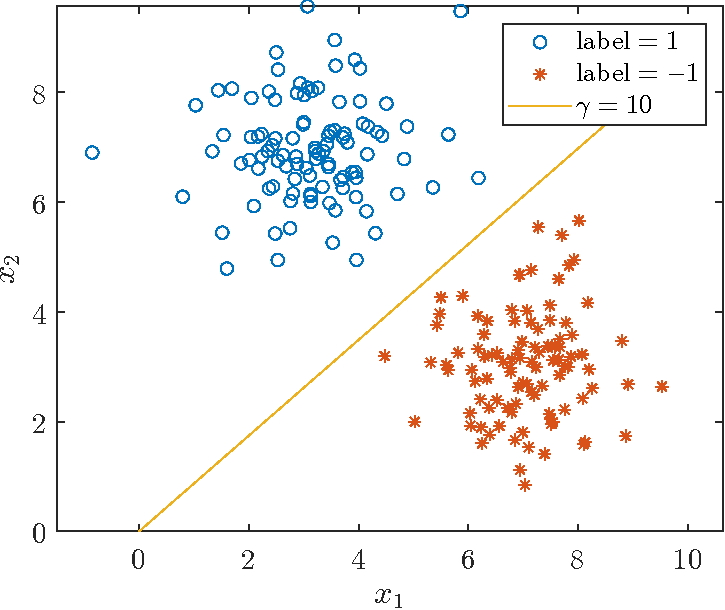
\includegraphics[width=8cm]{marginPrecep.pdf}
  \caption{感知器分类结果, margin 为 10}
  \label{fig:marginPrecep}
  \end{minipage}
  \begin{minipage}[t]{0.48\textwidth}
  \centering
  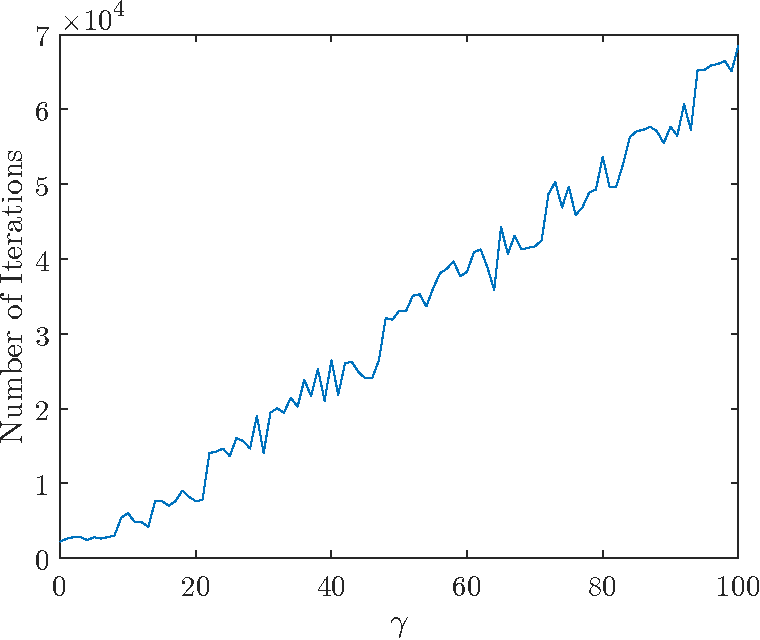
\includegraphics[width=8cm]{marginEffect.pdf}
  \caption{margin 大小对算法迭代次数的影响}
  \label{fig:marginEffect}
  \end{minipage}
\end{figure}

取 $\gamma=0,10,\dots,80$, 分别绘制分类边界如图 \ref{fig:marginEffect2} 所示, 可以看出分类边界的位置随着 $\gamma$ 的增大而改变, 分类边界到与其最近的数据点的距离随着 $\gamma$ 的增大而有所增大, 逐渐趋于两类之间居中的位置.

\begin{figure}[htbp]
  \centering
  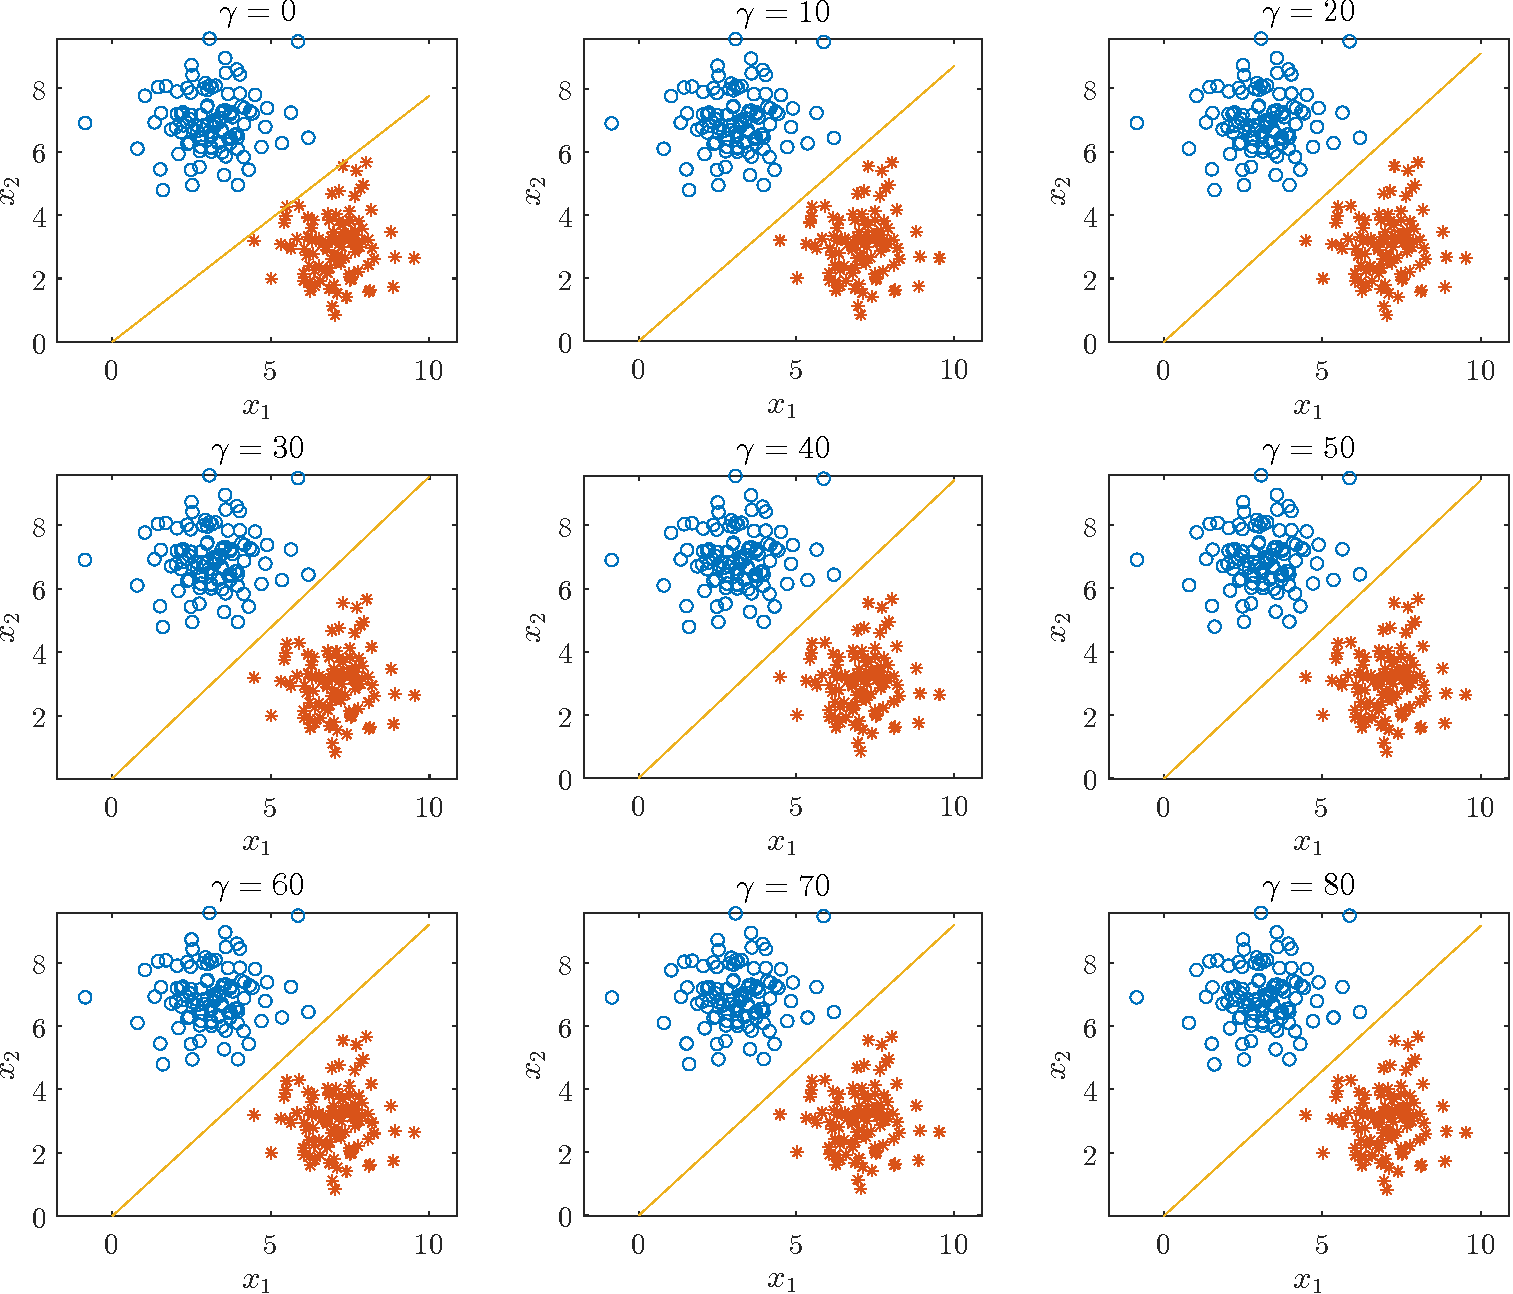
\includegraphics[width=17cm]{marginEffect2.pdf}
  \caption{感知器分类结果, margin 从 0 变化到 80}
  \label{fig:marginEffect2}
\end{figure}

\newpage
\section*{Proof of Single Sample Correction Algorithm}

4. Suppose we have $N$ points $x_i$ in $\mathbb{R}^p$ with class labels $\omega_i\in\{-1,1\}$. Prove that the perceptron algorithm converges to a separating hyperplane in finite steps:
\begin{itemize}
  \item Denoting a hyperplane by $f(x)=a_1^{\top}x+a_0=0$, or in more compact notation $a^{\top}y= 0$, where $y=(x,1)$ and $a=(a_1,a_0)$. Let $z_i=\dfrac{y}{\|y\|_2}$. Show that separability implies there exists a $a_{\mathrm{sep}}$ such that $\omega_ia_{\mathrm{sep}}^{\top}z_i\gs1$, $\forall~i=1,2,\dots,N$.
  \item Given a current $a_{\mathrm{old}}$, the Algorithm~\ref{alg:1} identifies a point $z_i$ that is misclassified, and produces the update $a_{\mathrm{new}} = a_{\mathrm{old}}+\omega_iz_i$. Show that $\|a_{\mathrm{new}}-a_{\mathrm{sep}}\|_2^2\ls\|a_{\mathrm{old}}-a_{\mathrm{sep}}\|_2^2-1$, and hence the algorithm converges to a separating hyperplane in no more than $\|a_{\mathrm{start}}-a_{\mathrm{sep}}\|_2^2$ steps. 
\end{itemize}

证明: 假设数据是线性可分的, 则 $\exists~\bar{a}\in\mathbb{R}^{p+1}$ 使得
\begin{equation}
  \omega_i\bar{a}^{\top}y_i>0,\quad \forall~i=1,2,\dots,N
\end{equation}

其中 $y_i=(x_i,1)$, 则 $\|y_i\|_2>0$, $\forall~i=1,2,\dots,N$, 所以
\begin{equation}
  \omega_i\bar{a}^{\top}\frac{y_i}{\|y_i\|_2}>0,\quad \forall~i=1,2,\dots,N
\end{equation}

令 $z_i=\dfrac{y_i}{\|y_i\|_2}$, 则有
\begin{equation}
  \omega_i\bar{a}^{\top}z_i>0,\quad \forall~i=1,2,\dots,N
\end{equation}

所以
\begin{equation}
  \omega_i\bar{a}^{\top}z_i\gs\min_{i}\{\omega_i\bar{a}^{\top}z_i\}>0,\quad \forall~i=1,2,\dots,N
\end{equation}

因此
\begin{equation}
  \frac{\omega_i\bar{a}^{\top}z_i}{\min_{i}\{\omega_i\bar{a}^{\top}z_i\}}\gs1,\quad \forall~i=1,2,\dots,N
\end{equation}

取
\begin{equation*}
  a_{\mathrm{sep}}=\frac{\bar{a}}{\min_{i}\{\omega_i\bar{a}^{\top}z_i\}}
\end{equation*}

则有
\begin{equation}
  \omega_ia_{\mathrm{sep}}^{\top}z_i\gs1,\quad \forall~i=1,2,\dots,N
\end{equation}

假设点 $z_i$ 被 $a_{\mathrm{old}}$ 错分, 即有
\begin{equation}
  \omega_ia_{\mathrm{old}}^{\top}z_i<0
\end{equation}

则算法下一步更新
\begin{equation}
  a_{\mathrm{new}} = a_{\mathrm{old}}+\omega_iz_i
\end{equation}

结合以上三式可得
\begin{equation}
  \begin{aligned}
    \|a_{\mathrm{new}}-a_{\mathrm{sep}}\|_2^2
    &=\|a_{\mathrm{old}}-a_{\mathrm{sep}}+\omega_iz_i\|_2^2\\
    &=\|a_{\mathrm{old}}-a_{\mathrm{sep}}\|_2^2+\|\omega_iz_i\|_2^2+2\omega_i(a_{\mathrm{old}}-a_{\mathrm{sep}})^{\top}z_i\\
    &=\|a_{\mathrm{old}}-a_{\mathrm{sep}}\|_2^2+1+2\omega_ia_{\mathrm{old}}^{\top}z_i-2\omega_ia_{\mathrm{sep}}^{\top}z_i\\
    &\ls\|a_{\mathrm{old}}-a_{\mathrm{sep}}\|_2^2+1+0-2\\
    &=\|a_{\mathrm{old}}-a_{\mathrm{sep}}\|_2^2-1
  \end{aligned}
\end{equation}

假设算法从 $a_{\mathrm{start}}$ 开始, 经 $n$ 步更新得到 $a^{(n)}$, 则由上式可知
\begin{equation}
  0\ls\|a^{(n)}-a_{\mathrm{sep}}\|_2^2\ls\|a^{(n-1)}-a_{\mathrm{sep}}\|_2^2-1\ls\dots\ls\|a_{\mathrm{start}}-a_{\mathrm{sep}}\|_2^2-n
\end{equation}

因此有
\begin{equation}
  n\ls\|a_{\mathrm{start}}-a_{\mathrm{sep}}\|_2^2
\end{equation}

即算法更新次数不会超过 $\|a_{\mathrm{start}}-a_{\mathrm{sep}}\|_2^2$, 所以算法不超过 $\|a_{\mathrm{start}}-a_{\mathrm{sep}}\|_2^2$ 步就会收敛到一个分离超平面.\qed

% Reference
% \begin{thebibliography}{1}
%   \bibitem{b1}{Flying pig. Deriving the conditional distributions of a multivariate normal distribution, 2012. \href{https://stats.stackexchange.com/questions/30588}{https://stats.stackexchange.com/questions/30588}}
% \end{thebibliography}

\end{document}
